\section{Hybrid impedance controller}
In the present section the hybrid impedance controller is presented. 
It allows to control the position expressed in work-space frame and the attitude 
with respect the work-space coordinate system of the end-effector while a contact 
force between the object and the SoftHand is regulated.
The position errors ($e_x$ and $e_y$) and the attitude error ($\vec{e}_{\Phi}$) respect the desired trajectory are given by
\[
\begin{split}
  &\ddot{e}_{x} + B_x \dot{e}_x + K_x e_x = \prescript{ws}{}{F}_x\\
  &\ddot{e}_{y} + B_y \dot{e}_y + K_y e_y = \prescript{ws}{}{F}_y\\
  &\ddot{\vec{e}}_{\Phi} + B_{\Phi} \dot{\vec{e}}_{\Phi} + K_{\Phi} \vec{e}_{\Phi} = \prescript{ws}{}{M}
\end{split}
\]
where $\prescript{ws}{}{F}_x$, $\prescript{ws}{}{F}_y$ and 
$\prescript{ws}{}{M}$ are the forces and torques
exchanged with the environment expressed in the workspace frame. 
While in the z-axis of the workspace frame the error respect must be minimized
\[
e_z \xrightarrow[t \to \infty]{} 0
\]

\subsection{Operational space state}
The control problem is to choose the input to cause the end-effector 
to execute a desired motion in task space while regulating the 
forces of interaction of the end-effector with the environment.
In order to develop the controller the operational space state is defined
\begin{equation}
  \label{eq:state_space}
  \prescript{ws}{}{\vec{x}} = 
  \begin{bmatrix}
    r_x & r_y & r_z & \psi & \theta & \phi
  \end{bmatrix}^T
\end{equation}
where $r_x$, $r_y$ and $r_z$ are the position vector of the palm 
of the hand expressed in workspace frame while $\psi$, $\theta$ and 
$\phi$ are the euler parametrization of the rotation 
$\prescript{ws}{}{R}_{ee}$ between the workspace frame and the end-effector frame
\[
\prescript{ws}{}{R}_{ee} = R_{ZYZ}(\psi, \theta, \phi) = R_{ZYZ}(\vec{\Phi})
\]
Finally suppose that it is possible command the second derivative of the state
\[
\prescript{ws}{}{\ddot{\vec{x}}} = \vec{a} = \dot{\vec{v}}
\]

\subsection{Research in force control}
The Hybrid impedance controller (HIC) combines two controller 
architectures, the hybrid position/force control and the impedance control.
The first one, firstly proposed by Raibert and Craing (cita), 
is based on the orthogonal task space decomposition and it 
allows to assign different control strategies to each 
Cartesian degree of freedom however it neglects the 
manipulator impedance in the interaction with the environment.
The impedance control considers the effects of the 
impedance in the interaction between of the robot and the 
environment but it does not allow to control directly the force trajectory.

\subsection{Modelling the Environment}
In order to develop the hybrid impedance control the each 
degree of freedom of the environment and the robot must 
be modelled. they are usually modelled as a linear spring $K$, 
which is sometimes in parallel with a dash-pot $B$. In general 
the robot and the environment systems are described on the 
low-frequency behaviour of the impedance using the ratio of the 
Laplace transform of the force and the velocity.
In the frequency domain the impedances can be expressed using a complex number
\begin{equation}
  \label{eq:impedance}
  Z(\omega)=R(\omega)+jX(\omega)
\end{equation}
where $R(\omega)$ is the real part and $X(\omega)$ the imaginary part.

As $\omega$ approaches zero, one of three things can happen to 
the magnitude of the environment's and robot's impedance. It can 
approach infinity, it can approach a non-zero finite number, 
or it can approach zero. 
The following classification is used:
\begin{itemize}
\item A system with impedance given by the equation \ref{eq:impedance} is \emph{inertial} IFF $\lim_{\omega \to 0}|Z(\omega)| = 0$ (Fig. \ref{fig:type_of_impedances}.a)
\item A system with impedance given by the equation \ref{eq:impedance} is \emph{resistive} IFF $\lim_{\omega \to 0}|Z(\omega)| = c$ where $0<c<\infty$ (Fig. \ref{fig:type_of_impedances}.b)
\item A system with impedance given by the equation \ref{eq:impedance} is \emph{capacitive} IFF $\lim_{\omega \to 0}|Z(\omega)| = \infty$ (Fig. \ref{fig:type_of_impedances}.c)
\end{itemize}
\begin{figure}[h]
  \centering
  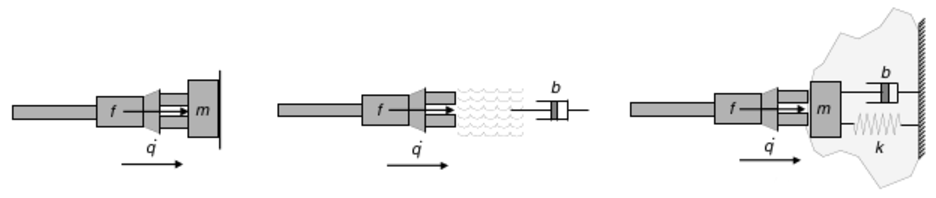
\includegraphics[scale=0.9]{type_of_impedances.pdf}
  \caption{Type of impedance. \label{fig:type_of_impedances}}
\end{figure}

Capacitive, inertial and resistive systems are usually described in terms of 
Norton and Thèvenin equivalents. A capacitive system is 
represented by an impedance in parallel with a flow source (Norton); 
an inertial system is represented by impedance in series with an 
effort source (Thévenin) and a resistive system 
can be either represented by a Thèvenin or Norton equivalents.

\subsection{Duality principles}
Once the environment has been properly modelled, the 
desired manipulator response may be determined. A fundamental goal for 
designing a controller is zero steady-state error to a step 
input. This will be obtained if we adhere to the 
following duality principle.
\begin{theorem}
  The manipulator should be controlled to respond as the dual of the environment.
\end{theorem}
This principle is most easily described in terms of Norton and Thèvenin equivalents.
An inertial environment, represented using Thèvenin equivalent (Fig. \ref{fig:position_control_model}), is controlled by a manipulator represented by a non-inertial impedance.
\begin{figure}[h]
  \centering
  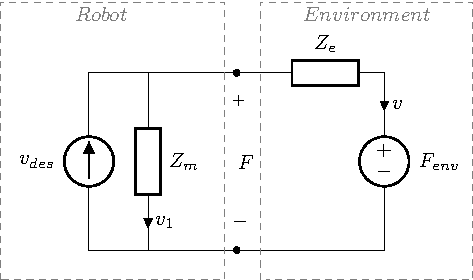
\includegraphics[scale=0.9]{position_control_model.pdf}
  \caption{Inertial environment. \label{fig:position_control_model}}
\end{figure}
Using the superposition principle the current (velocity) $v$ can be evaluated
\begin{equation}
  \label{eq:position_control_circuit}
  v = \frac{Z_m(s)}{Z_m(s) + Z_e(s)}v_{des} - 		\frac{F_{env}}{Z_e + Z_m}
\end{equation}
and the steady state error, assuming no environments input ($F_{env} \equiv 0$) is equal to 
\[
e_{ss} \Big|_{F_{env}(t) \equiv 0} = \lim_{s \to 0}(v - v_{des}) = \frac{-Z_e(0)}{Z_m(0) + Z_e(0)}
\]
if the environment is inertial ($|Z_e(0)| = 0$) and the manipulator is non-inertial ($Z_m(0) \neq 0$) 
\[
e_{ss} \Big|_{F_{env}(t) \equiv 0} = 0
\]
So inertial environments are position controlled with a non-inertial manipulator impedances.

A capacitive environment, represented using Norton equivalent (Fig. \ref{fig:force_control_model}), 
is controlled by a manipulator represented by a 
non-capacitive impedance.
\begin{figure}[h]
  \centering
  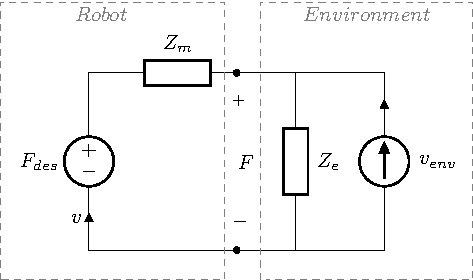
\includegraphics[scale=0.9]{force_control_model.pdf}
  \caption{Capacitive environment. \label{fig:force_control_model}}
\end{figure}
Using the superposition principle the effort $F$ can be evaluated
\begin{equation}
  \label{eq:force_control_circuit}
  F = \frac{Z_e(s)}{Z_m(s) + Z_e(s)}F_{des} + \frac{Z_e Z_m}{Z_m + Z_e} V_{env}
\end{equation}

and the steady state error, assuming no environments input ($v_{env} \equiv 0$) is equal to 
\[
e_{ss} \Big|_{v_{env}(t) \equiv 0} = \lim_{s \to 0}(F - F_{des}) = \frac{-Z_m(0)}{Z_m(0) + Z_e(0)}
\]
if the environment is capacitive ($Z_e(0) \rightarrow \infty$) and the manipulator is non-capacitive ($Z_m(0) < \infty$)
\[
e_{ss} \Big|_{v_{env}(t) \equiv 0} = 0
\]
So capacitive environments are force controlled with non-capacitive manipulator impedances.

\subsubsection{Position control}
The transfer function for the position-controlled circuit given in the Equation \ref{eq:position_control_circuit} can be realized be feedback of the contact force,
combined with information about the desired acceleration for the
manipulator. Figure \ref{fig:position_control_feedback} shows a block diagram of the position-control implementation
\begin{figure}[h]
  \centering
  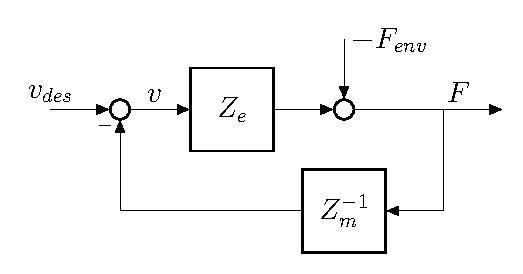
\includegraphics[scale=0.9]{position_control_feedback.pdf}
  \caption{Position control feedback. \label{fig:position_control_feedback}}
\end{figure}
where the commanded acceleration $a$ is given by
\[
a = \frac{\mathrm{d}}{\mathrm{d}t} \left(v_{des} - \frac{F}{Z_m}\right)
\]
in practise, the control $a$ can be obtained without differentiators and using only the measured force $F$ the end-effector position $x$ and velocity $\dot{x}$ if the robot impedance is given by
\[
Z_m = Ms + \tilde{Z}_{m}
\]
The position control law can be written using the following form
\begin{equation}
  \label{eq:position_law}
  a = \dot{v}_{des} + \frac{(v_{des} - v)\tilde{Z}_m}{M} - \frac{F}{M}
\end{equation}

\subsubsection{Force control}
The transfer function for the force-controlled circuit, showed in Equation \ref{eq:force_control_circuit}, can be realized by feedback of the force signal.
Figure \ref{fig:force_control_feedback} shows a block diagram of the force-control implementation
\begin{figure}[h]
  \centering
  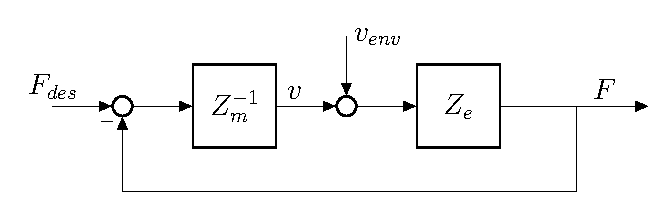
\includegraphics[scale=0.9]{force_control_feedback.pdf}
  \caption{Position control feedback. \label{fig:force_control_feedback}}
\end{figure}
where the acceleration $a$ is given by
\[
a = \frac{\mathrm{d}}{\mathrm{d}t} \left(\frac{F - F_{des}}{Z_m} \right)
\]
and the force $F$ is measured by a force/torque sensor.
As done before for position control DoF $a$ can be obtained without differentiators if
\[
Z_m = Ms + \tilde{Z}_{m}
\]
The force control law can be written using the following form
\begin{equation}
  \label{eq:force_law}
  a = \frac{1}{M} (F - F_{des}) - \frac{1}{M}( \tilde{Z}_m v)
\end{equation}

\subsection{a}
For the problem presented in the introduction of 
this section the robot's impedances regarding the position and DoF are given by
\[
\begin{split}
  &Z_{m,p} = M_p s + \tilde{Z}_{m,p} = M_p s + B_p + \frac{K_p}{s}\\
  &Z_{m,a} = M_a s + \tilde{Z}_{m,a} = M_a s + B_a + \frac{K_a}{s}
\end{split}
\]
and the controller laws are 
\[
\begin{split}
  &a_{p} = a_{des,p} + \frac{B_p}{M_p} (v_{des,p} - v_p) + \frac{K_p}{M_p} (x_{des,p} - x_p) - \frac{F_p}{M_p}\\
  &a_a = a_{des,a} + \frac{B_a}{M_a} (v_{des,a} - v_a) + \frac{K_a}{M_a} (x_{des,a} - x_a) - \frac{F_a}{M_a}
\end{split}
\]
while for the force controller the impedance is given by
\[
Z_{m,f} = M_f s + \tilde{Z}_{m,f} = M_f s + B_f
\]
and the controller law is
\[  
a_{f} = M_f^{-1}((f_{des} - f) - B_f v_z)
\]
In principle a position control law and a force control law could be assign for each DoF and a 
selection matrix $S$ is used to separate the force-controlled and position-controlled reciprocal subspaces
\[
\vec{a} = S 
\begin{bmatrix}
  \vec{a}_p \\
  \vec{a}_a
\end{bmatrix} + (I - S) \vec{a}_f
\]
where the vector $\vec{a}_p$ and $\vec{a}_a$ are the position and attitude control laws
\[
\begin{split}
  &\vec{a}_p = 
  \begin{bmatrix}
    a_{p,x} & a_{p,y} & a_{p,z}
  \end{bmatrix}^T\\
  &\vec{a}_a = 
  \begin{bmatrix}
    a_{a, \psi} & a_{a, \theta} & a_{a, \phi}
  \end{bmatrix}^T
\end{split}
\]
the vector $\vec{a}_f$ is the force/torque controller vector
\[
\vec{a}_f = 
\begin{bmatrix}
  a_{f,x} & a_{f,y} & a_{f,z} & a_{f, \psi} & a_{f, \theta} & a_{f, \phi}
\end{bmatrix}^T
\]
and $S$ is the selection matrix that is in this specific case
\[
S =
\begin {bmatrix}
  1 & 0 & 0 & 0 & 0 & 0\\
  0 & 1 & 0 & 0 & 0 & 0\\
  0 & 0 & 0 & 0 & 0 & 0\\
  0 & 0 & 0 & 1 & 0 & 0\\
  0 & 0 & 0 & 0 & 1 & 0\\
  0 & 0 & 0 & 0 & 0 & 1\\
\end {bmatrix}
\]
The resulting control law is
\[
\begin{cases}
  a_x = \ddot{r}_{x,des} + B_x (\dot{r}_{x,des} - \dot{r}_x) + K_x (r_{x,des} - r_x) - F_x \\
  a_y = \ddot{r}_{y,des} + B_y (\dot{r}_{y,des} - \dot{r}_y) + K_y (r_{y,des} - r_y) - F_y \\
  a_z = - B_f \dot{r}_z + K_f(F_{z,des} - F_z) \\
  a_{\psi} = \ddot{\psi}_{des} + B_{\psi} (\dot{\psi}_{des} - \dot{\psi}) + K_{\psi} (\psi_{des} - \psi) \\
  a_{\theta} = \ddot{\theta}_{des} + B_{\theta} (\dot{\theta}_{des} - \dot{\theta}) + K_{\theta} (\theta_{des} - \theta) \\
  a_{\phi} = \ddot{\phi}_{des} + B_{\phi} (\dot{\phi}_{des} - \dot{\phi}) + K_{\phi} (\phi_{des} - \phi)
\end{cases}
\]
where the desired trajectories regarding the position and the attitude are $5^\text{th}$ order polynomials
\[
s(t) = a_5 t^5 + a_4 t^4 + a_3 t^3 + a_2 t^2 +a_1 t + a_0
\]
with the following boundary condition
\[
\begin{split}
  &s(0) = s_0 \quad \dot{s}(0) = 0 \quad \ddot{s}(0) = 0\\
  &s(t_f) = s_f \quad \dot{s}(t_f) = 0 \quad \ddot{s}(t_f) = 0
\end{split}
\]
while the reference force function is a $3^\text{th}$ order polynomial
\[
s(t) = a_3 t^3 + a_2 t^2 +a_1 t + a_0
\] 
with the following boundary condition
\[
\begin{split}
  &s(0) = s_0 \quad \dot{s}(0) = 0\\
  &s(t_f) = s_f \quad \dot{s}(t_f) = 0
\end{split}
\]
\newpage
